% Auto-generated LaTeX Figures Snippet

\begin{figure}[h]
\centering
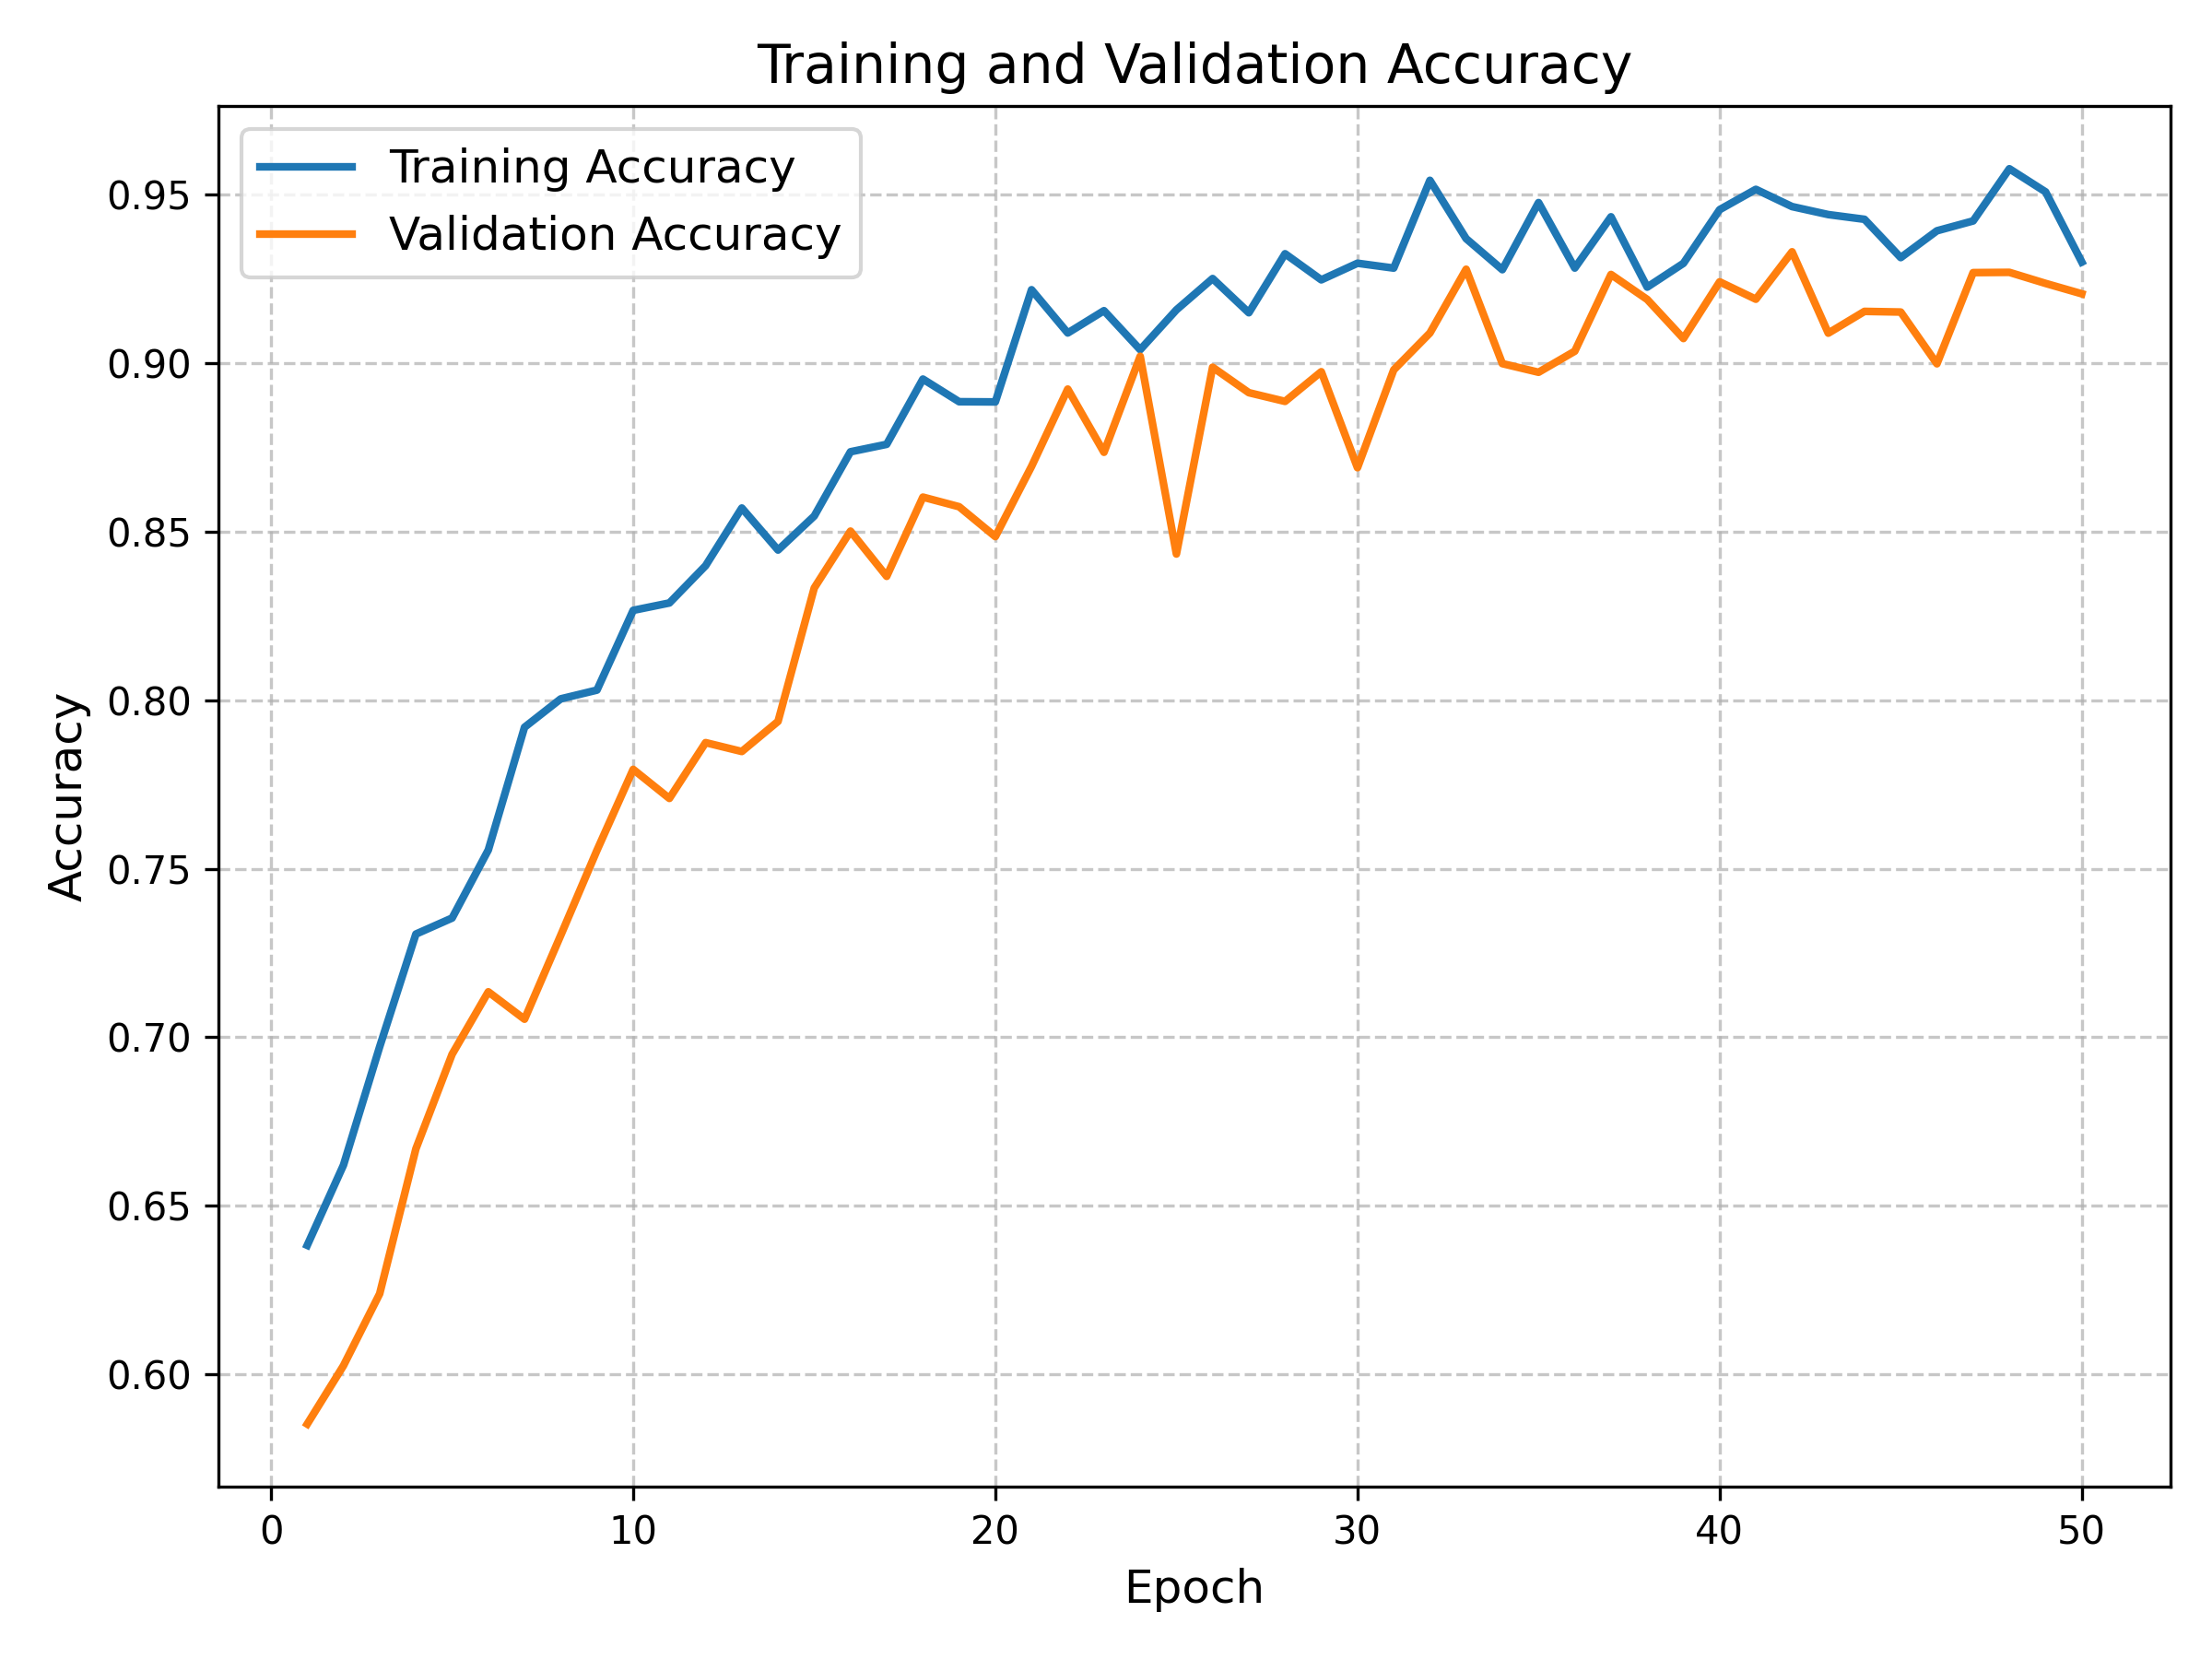
\includegraphics[width=0.8\textwidth]{figures/accuracy_plot.png}
\caption{Training and Validation Accuracy over Epochs}
\label{fig:accuracy-plot}
\end{figure}

\begin{figure}[h]
\centering
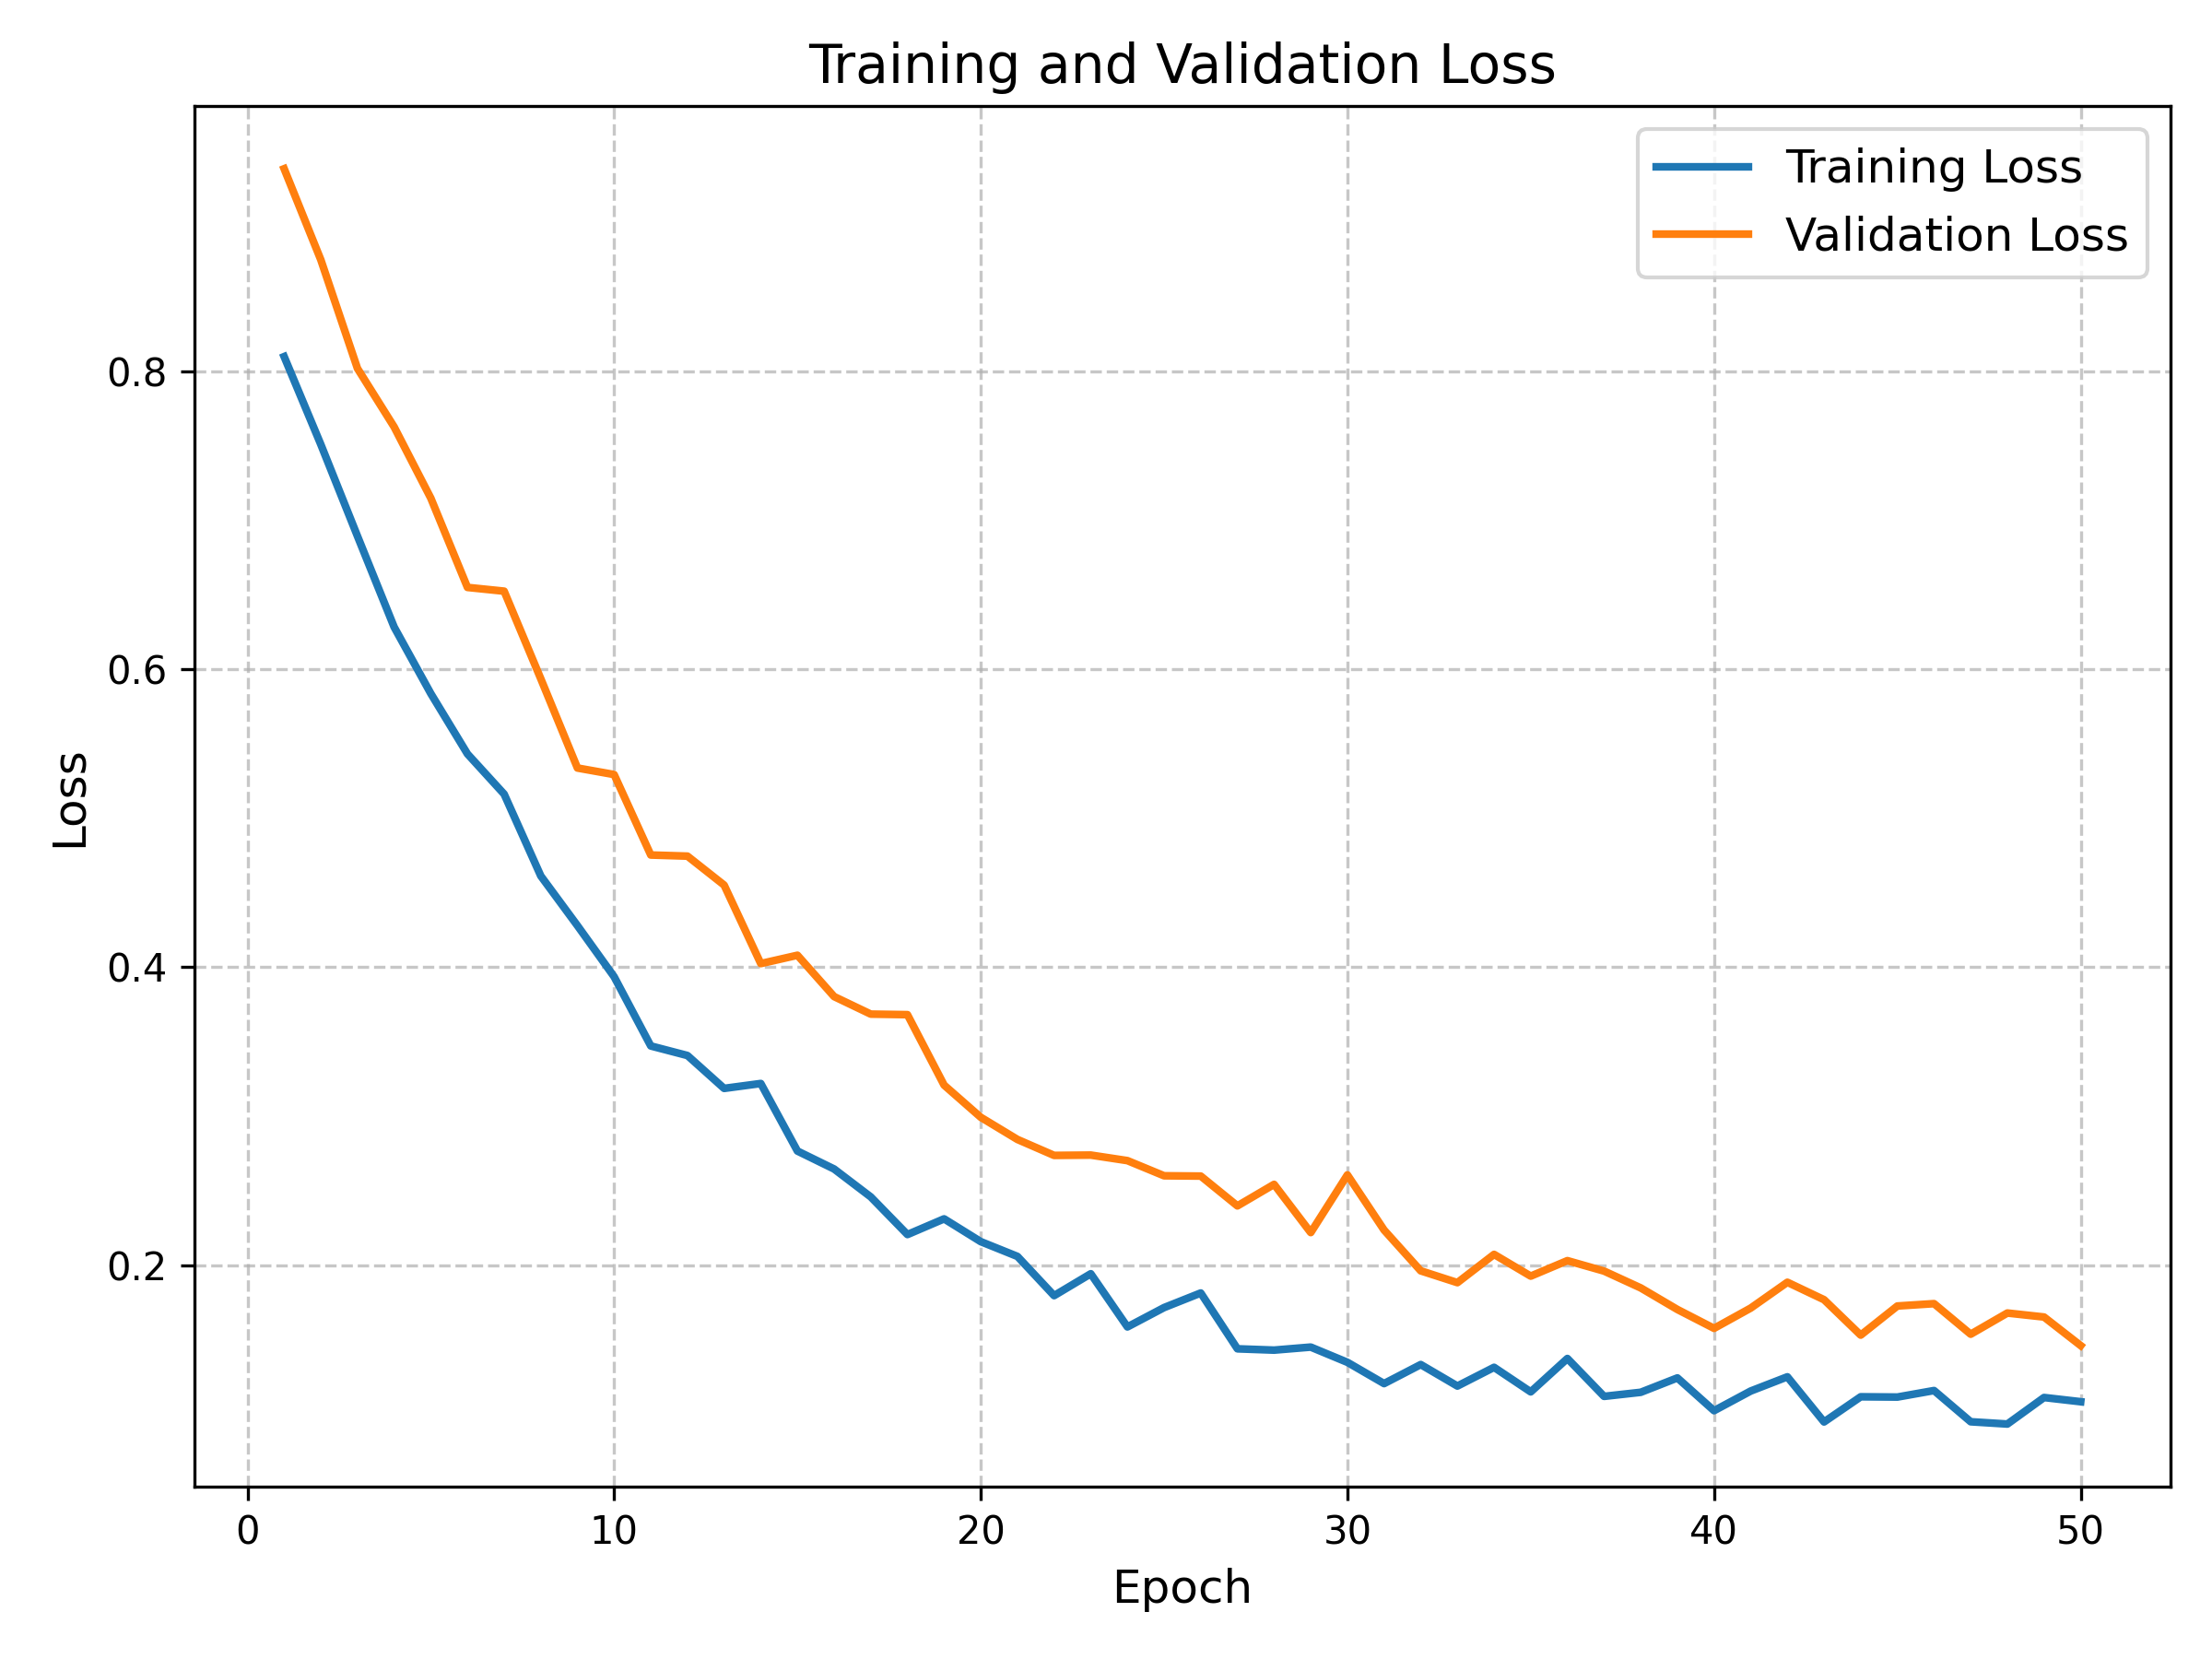
\includegraphics[width=0.8\textwidth]{figures/loss_plot.png}
\caption{Training and Validation Loss over Epochs}
\label{fig:loss-plot}
\end{figure}

\begin{figure}[h]
\centering
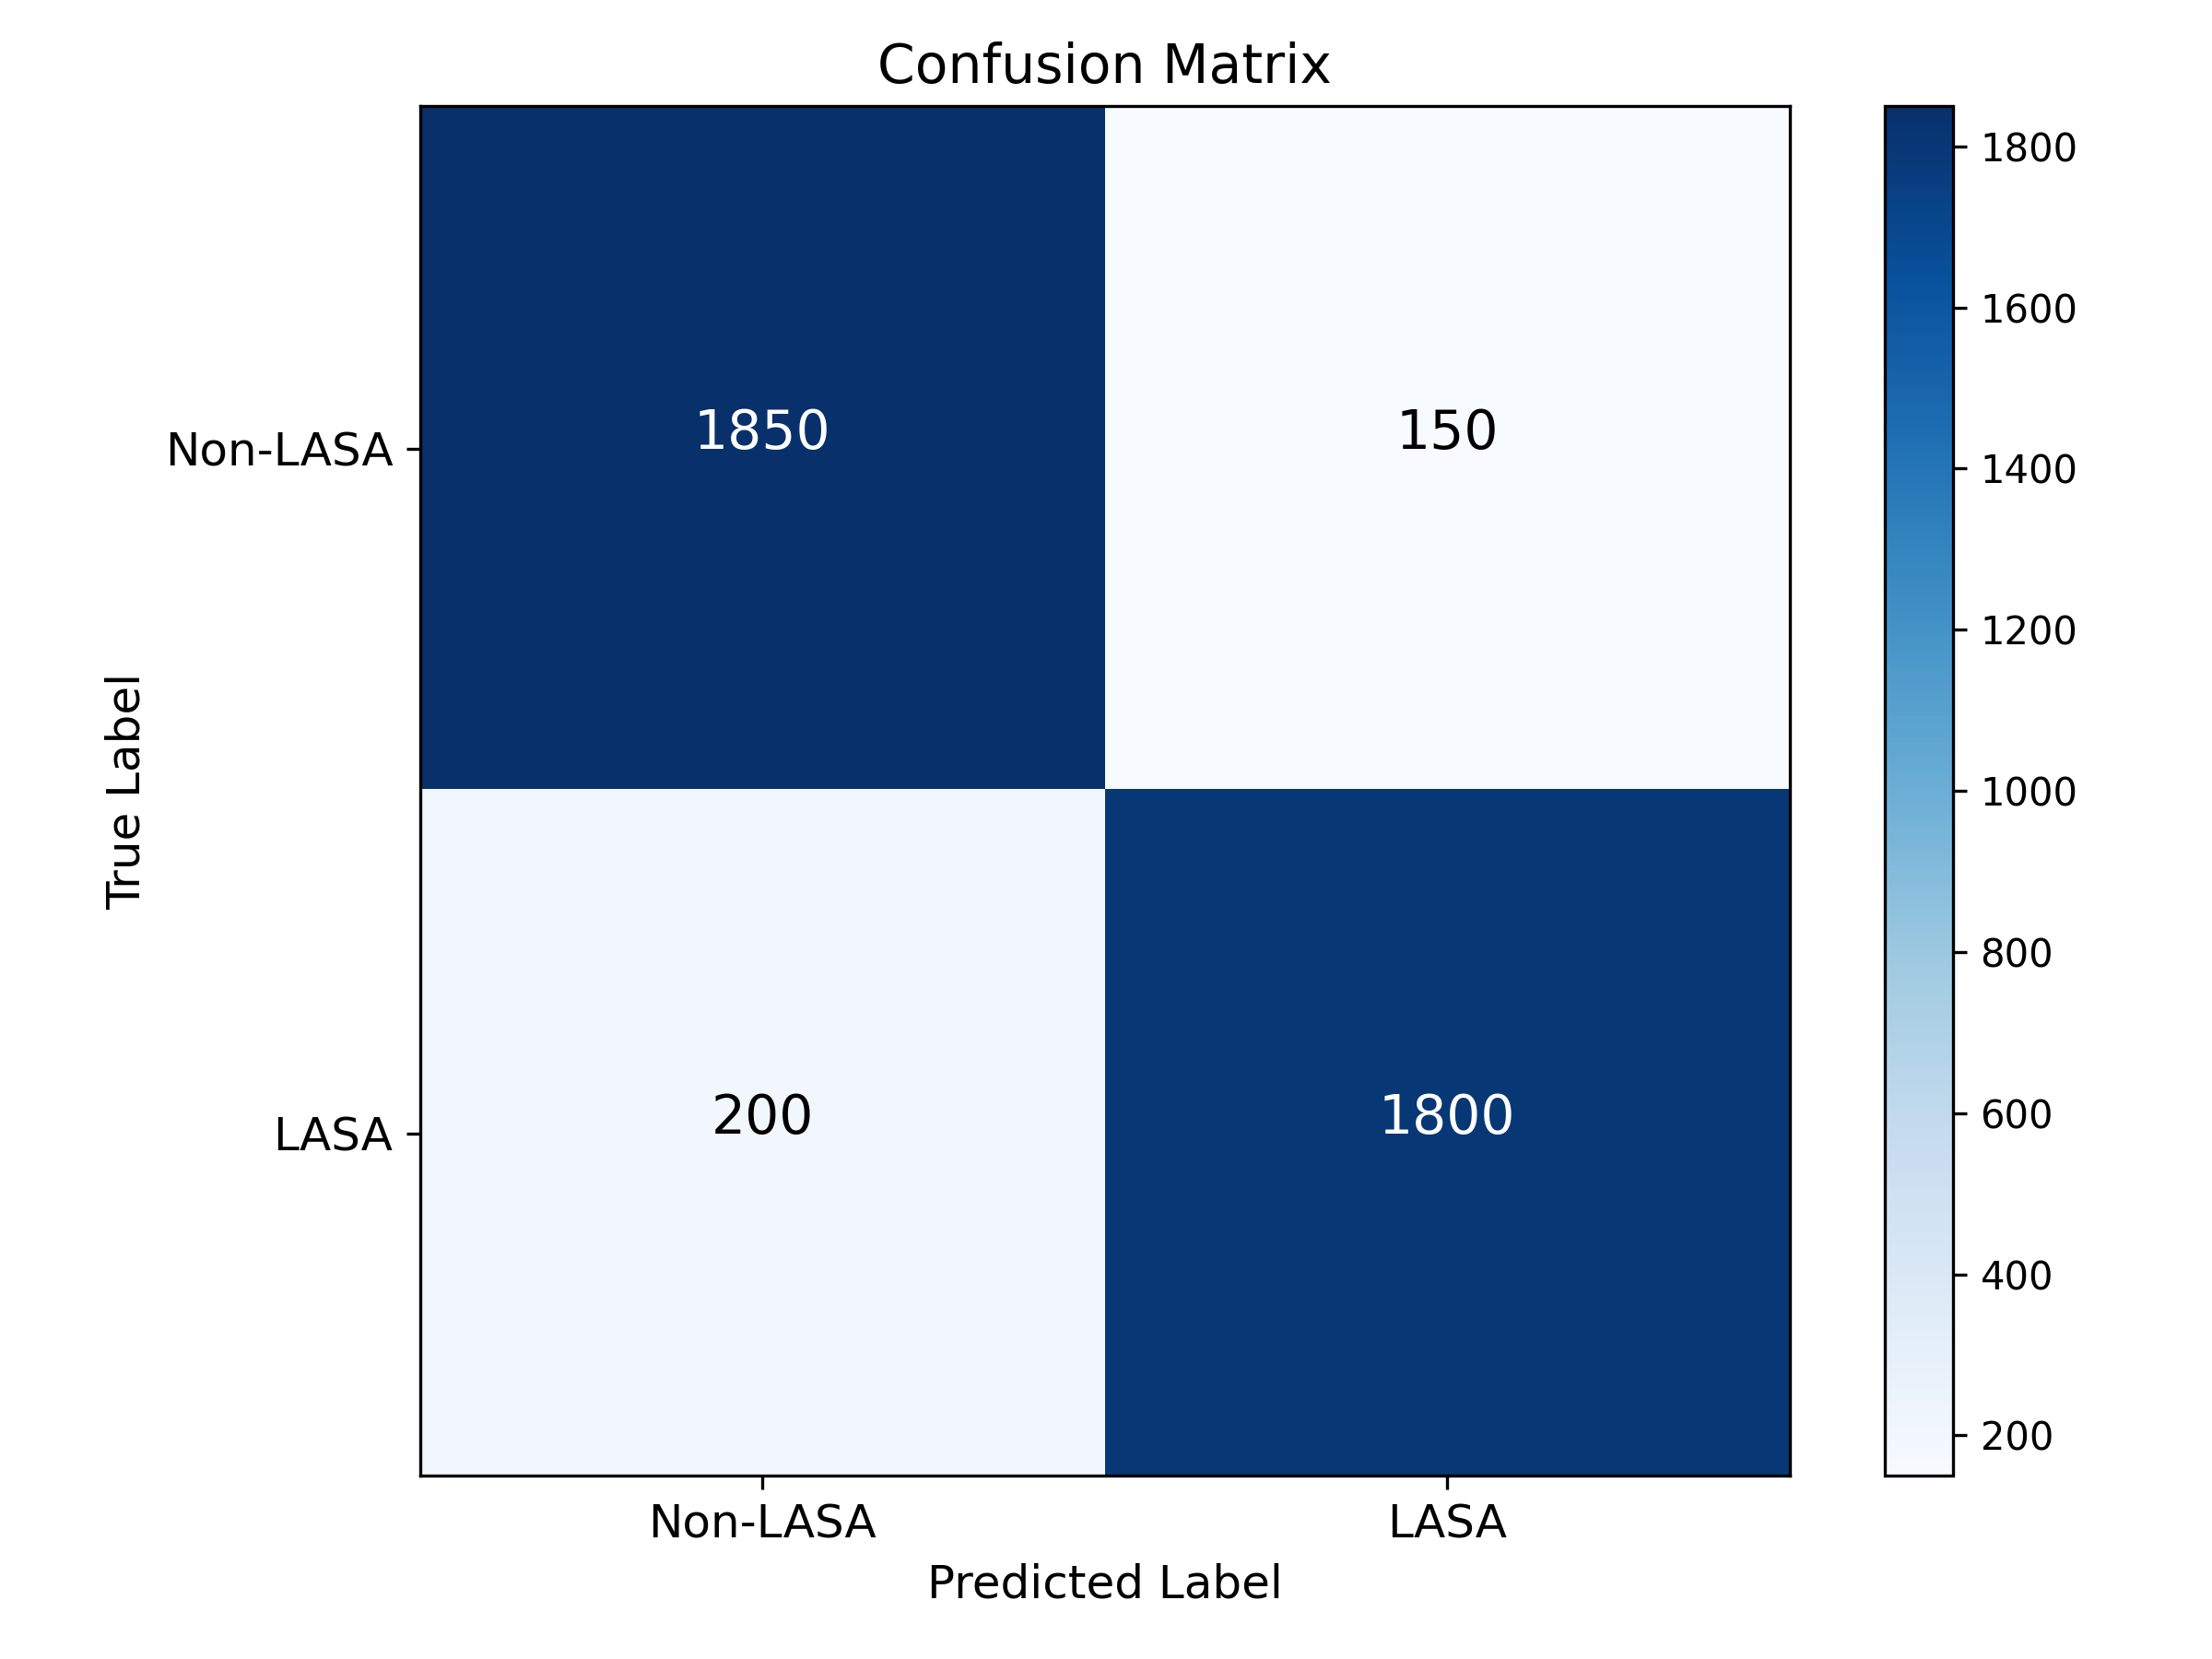
\includegraphics[width=0.8\textwidth]{figures/confusion_matrix.png}
\caption{Confusion Matrix of the Best Performing Model}
\label{fig:confusion-matrix}
\end{figure}

\begin{figure}[h]
\centering
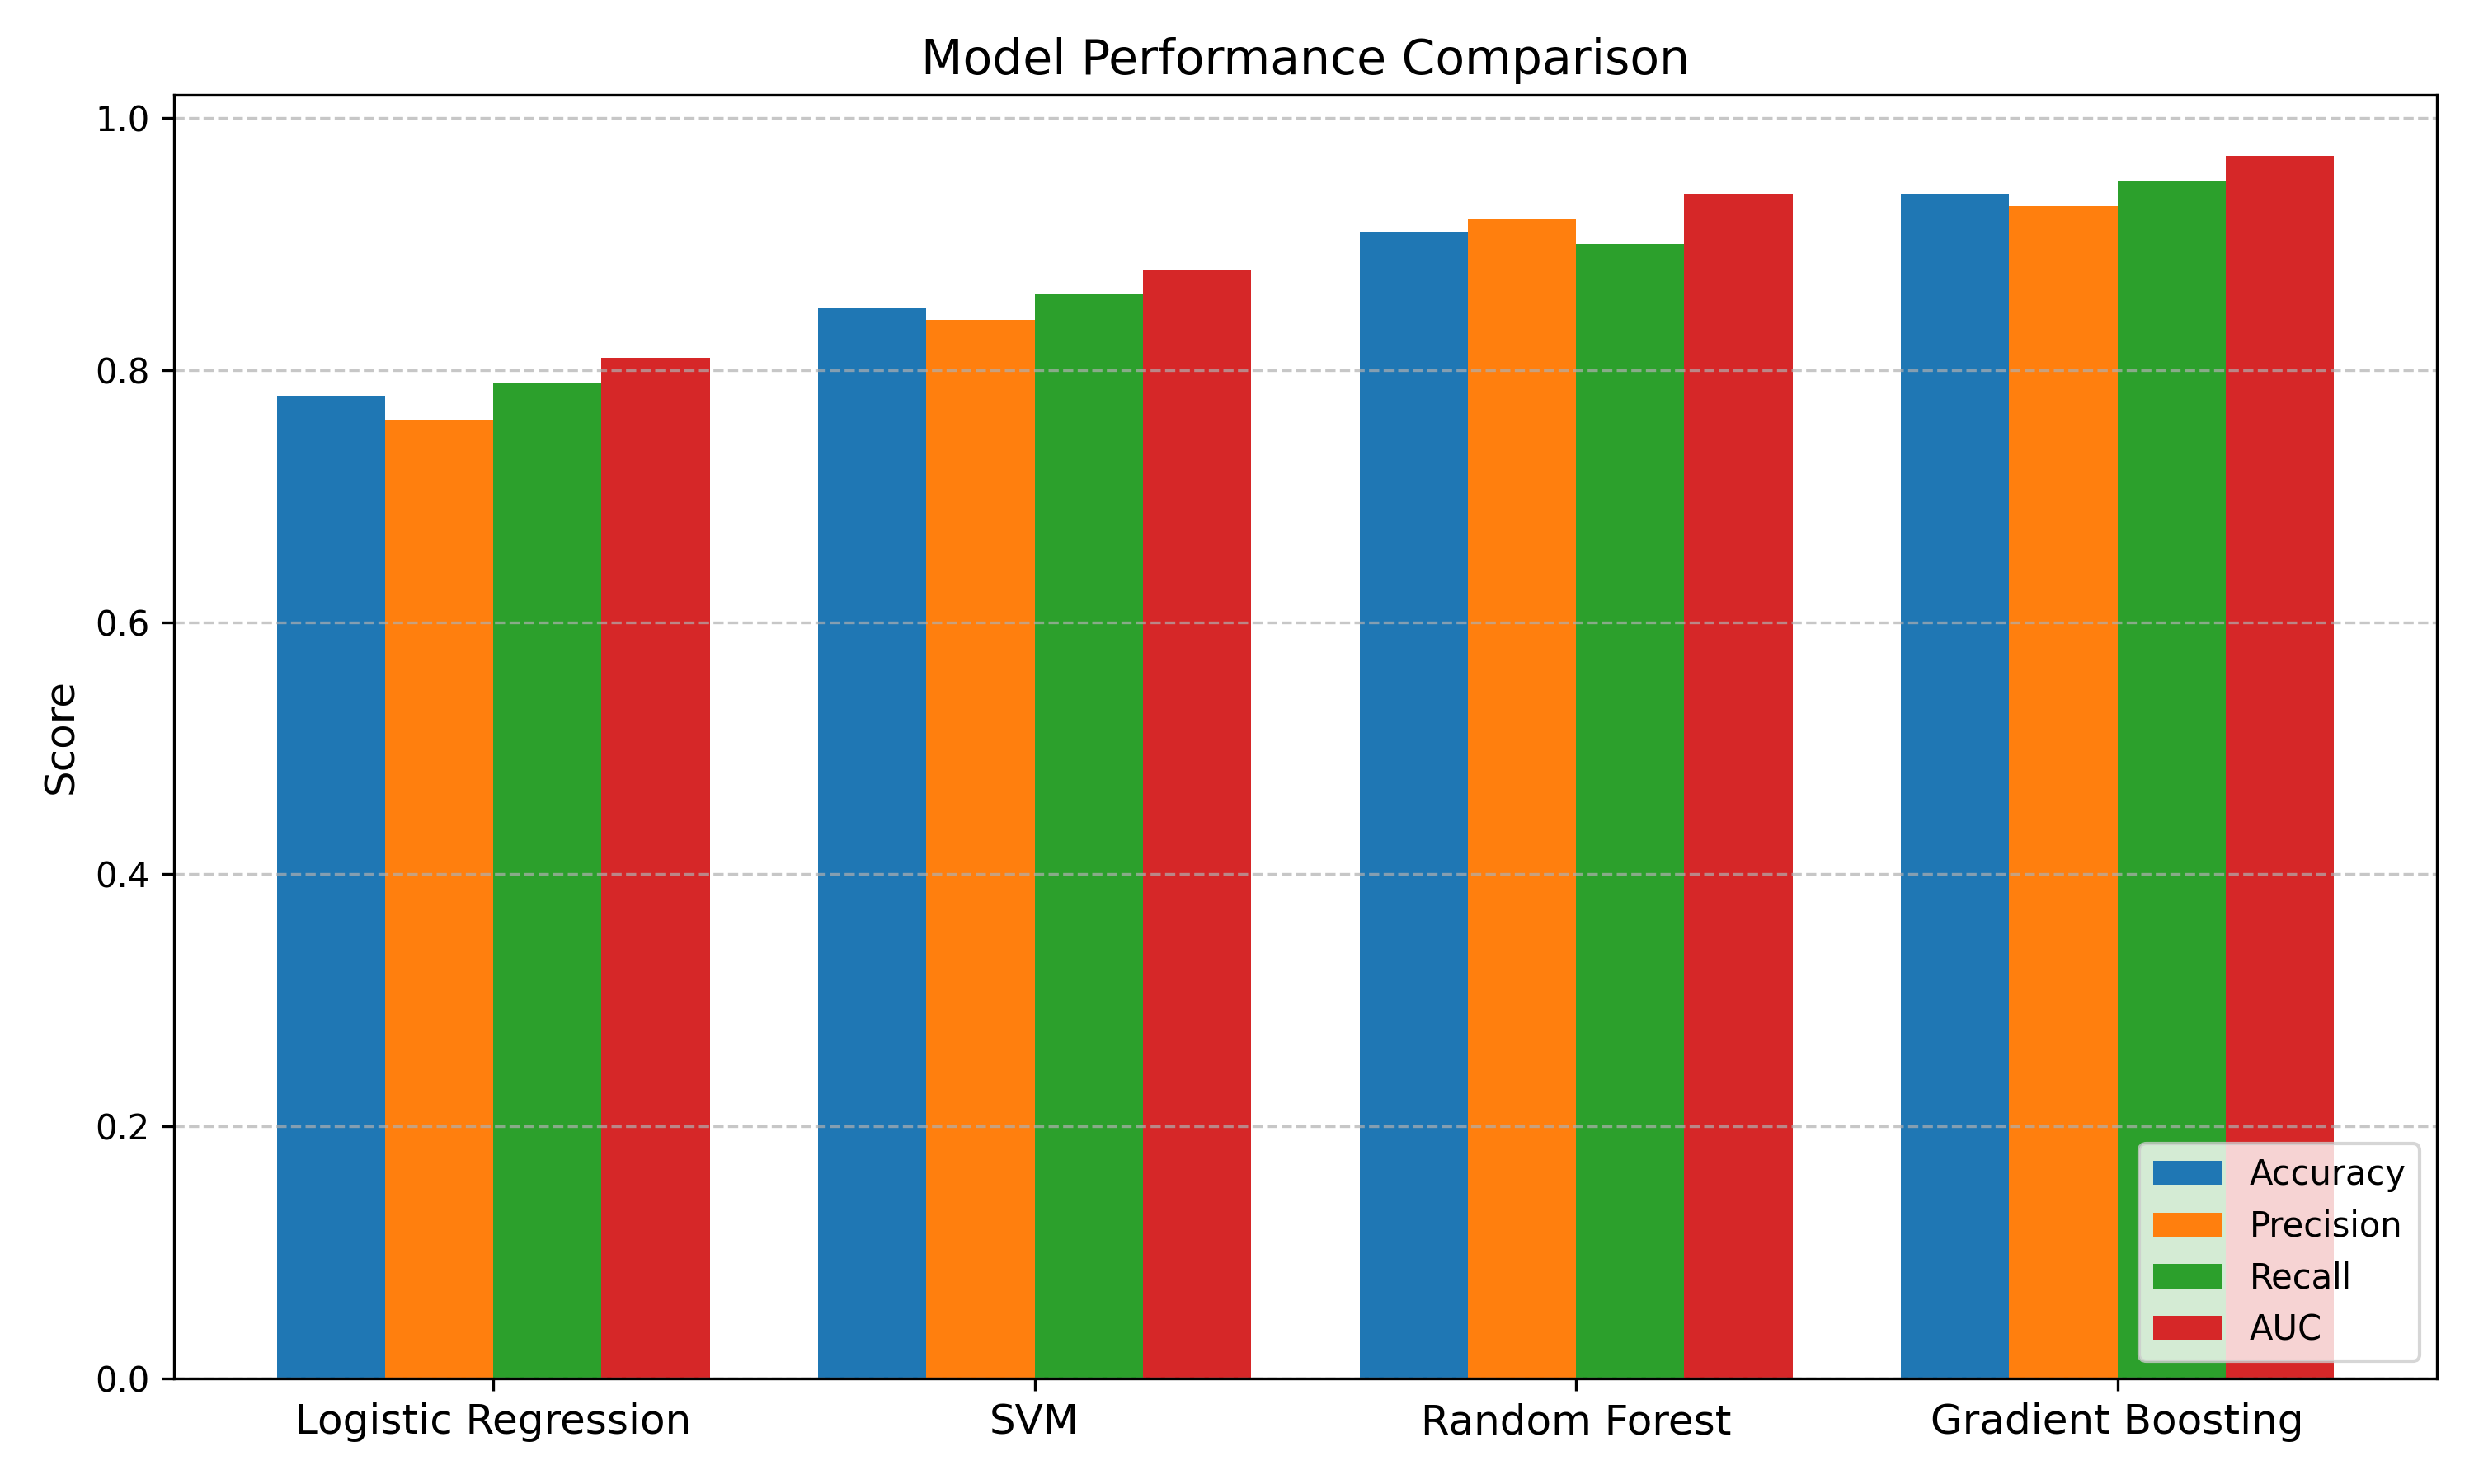
\includegraphics[width=0.8\textwidth]{figures/model_comparison.png}
\caption{Performance Comparison Across Different Machine Learning Models}
\label{fig:model-comparison}
\end{figure}

\begin{figure}[h]
\centering
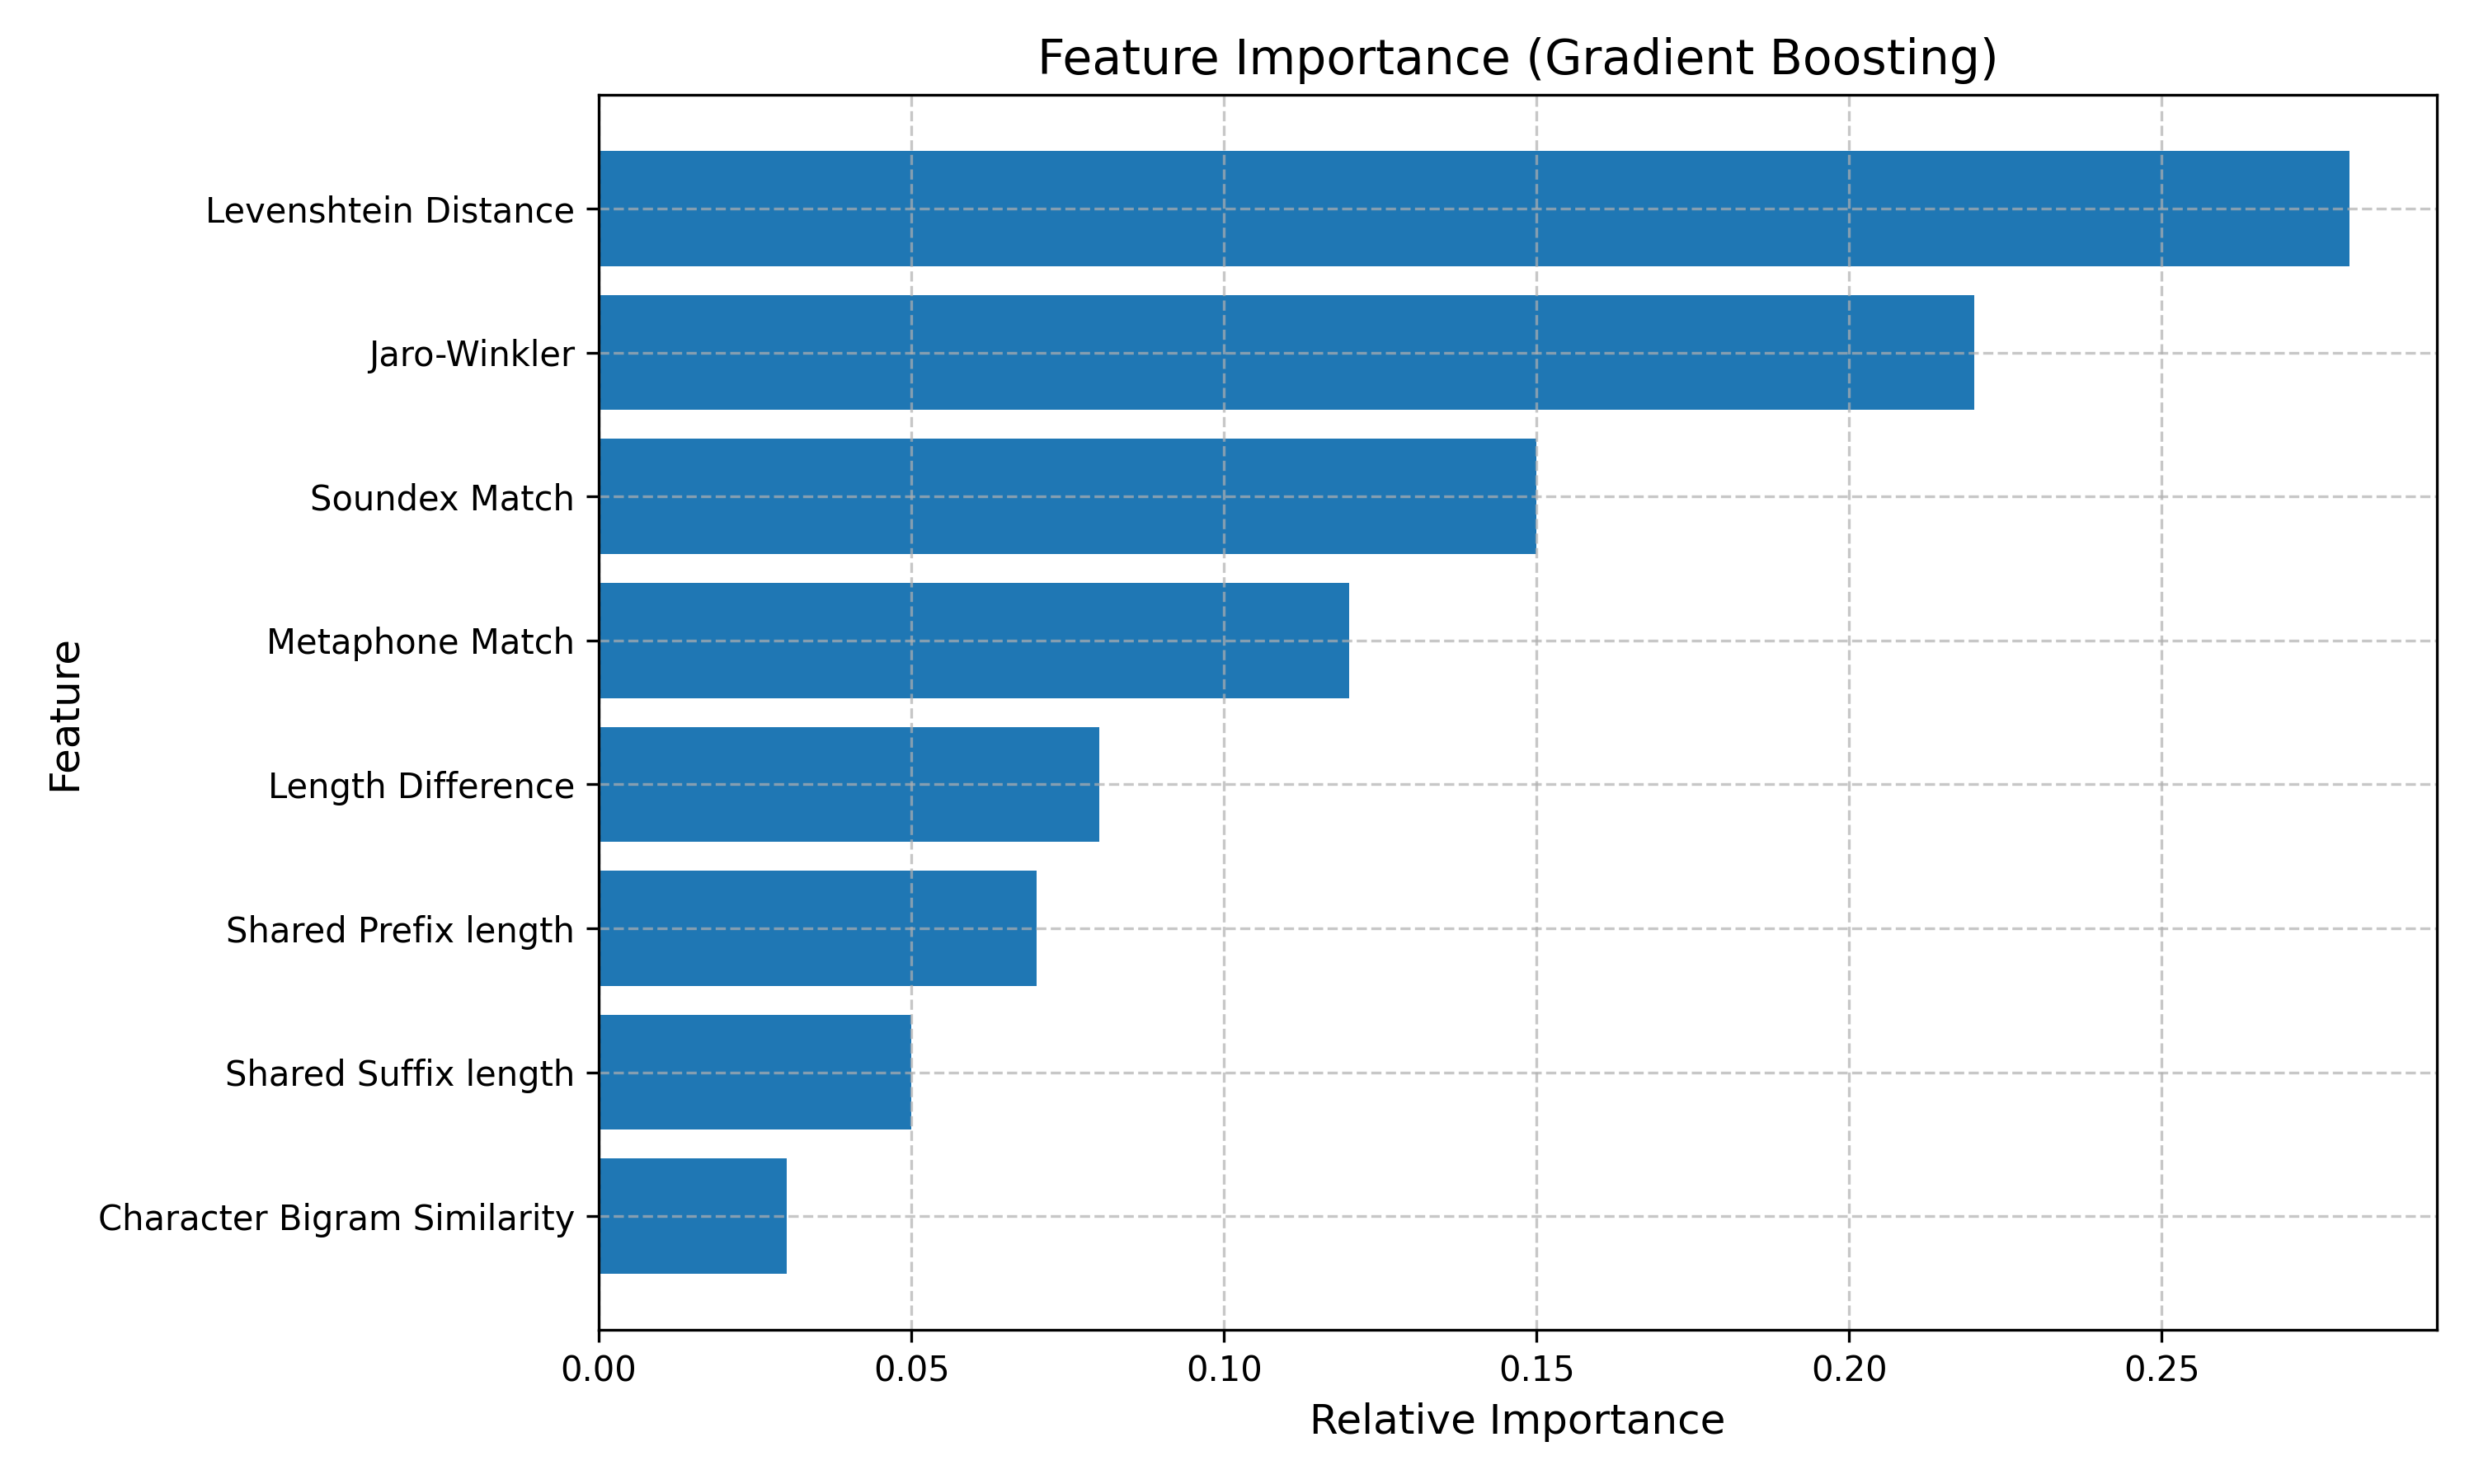
\includegraphics[width=0.8\textwidth]{figures/feature_importance.png}
\caption{Relative Importance of Engineered Features}
\label{fig:feature-importance}
\end{figure}

\begin{figure}[h]
\centering
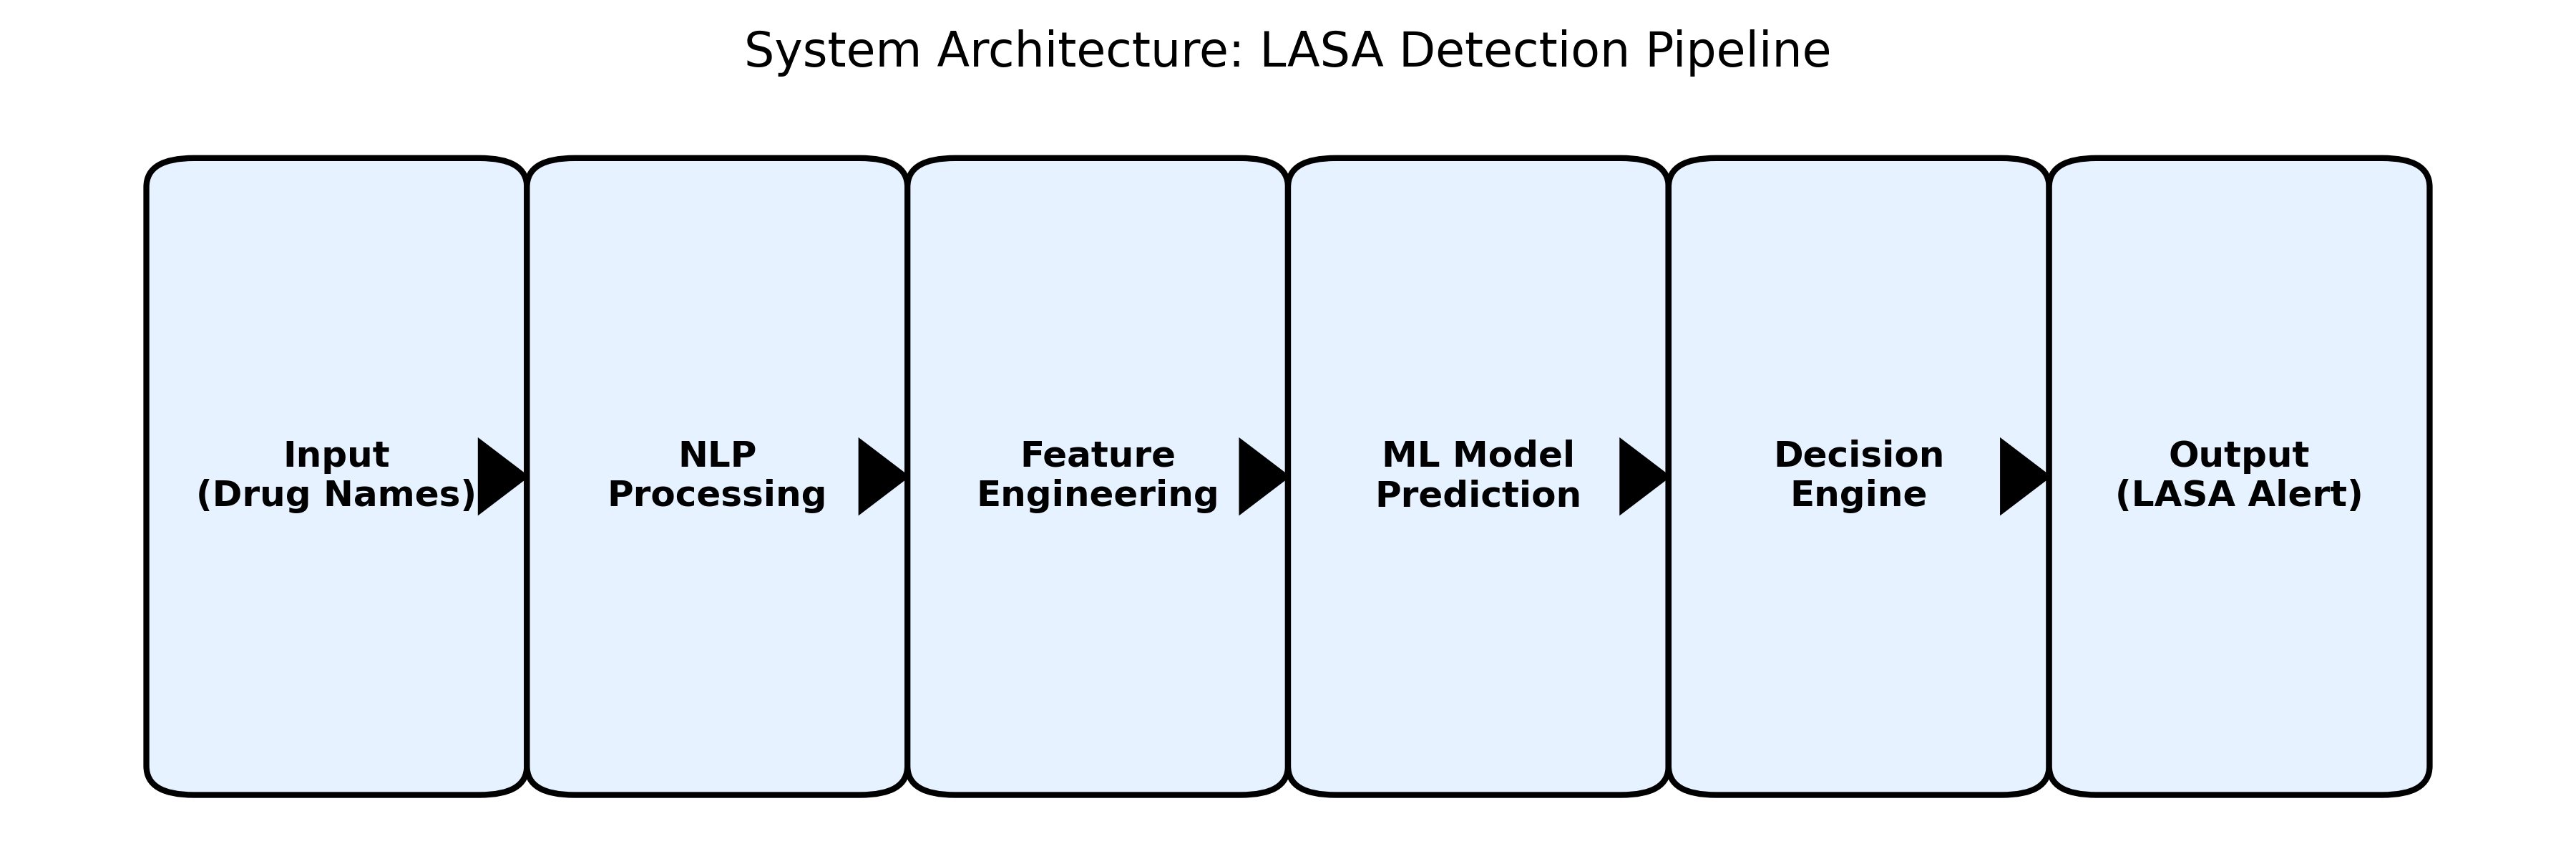
\includegraphics[width=0.8\textwidth]{figures/system_architecture.png}
\caption{System Architecture of the LASA Detection Pipeline}
\label{fig:system-architecture}
\end{figure}

\begin{figure}[h]
\centering
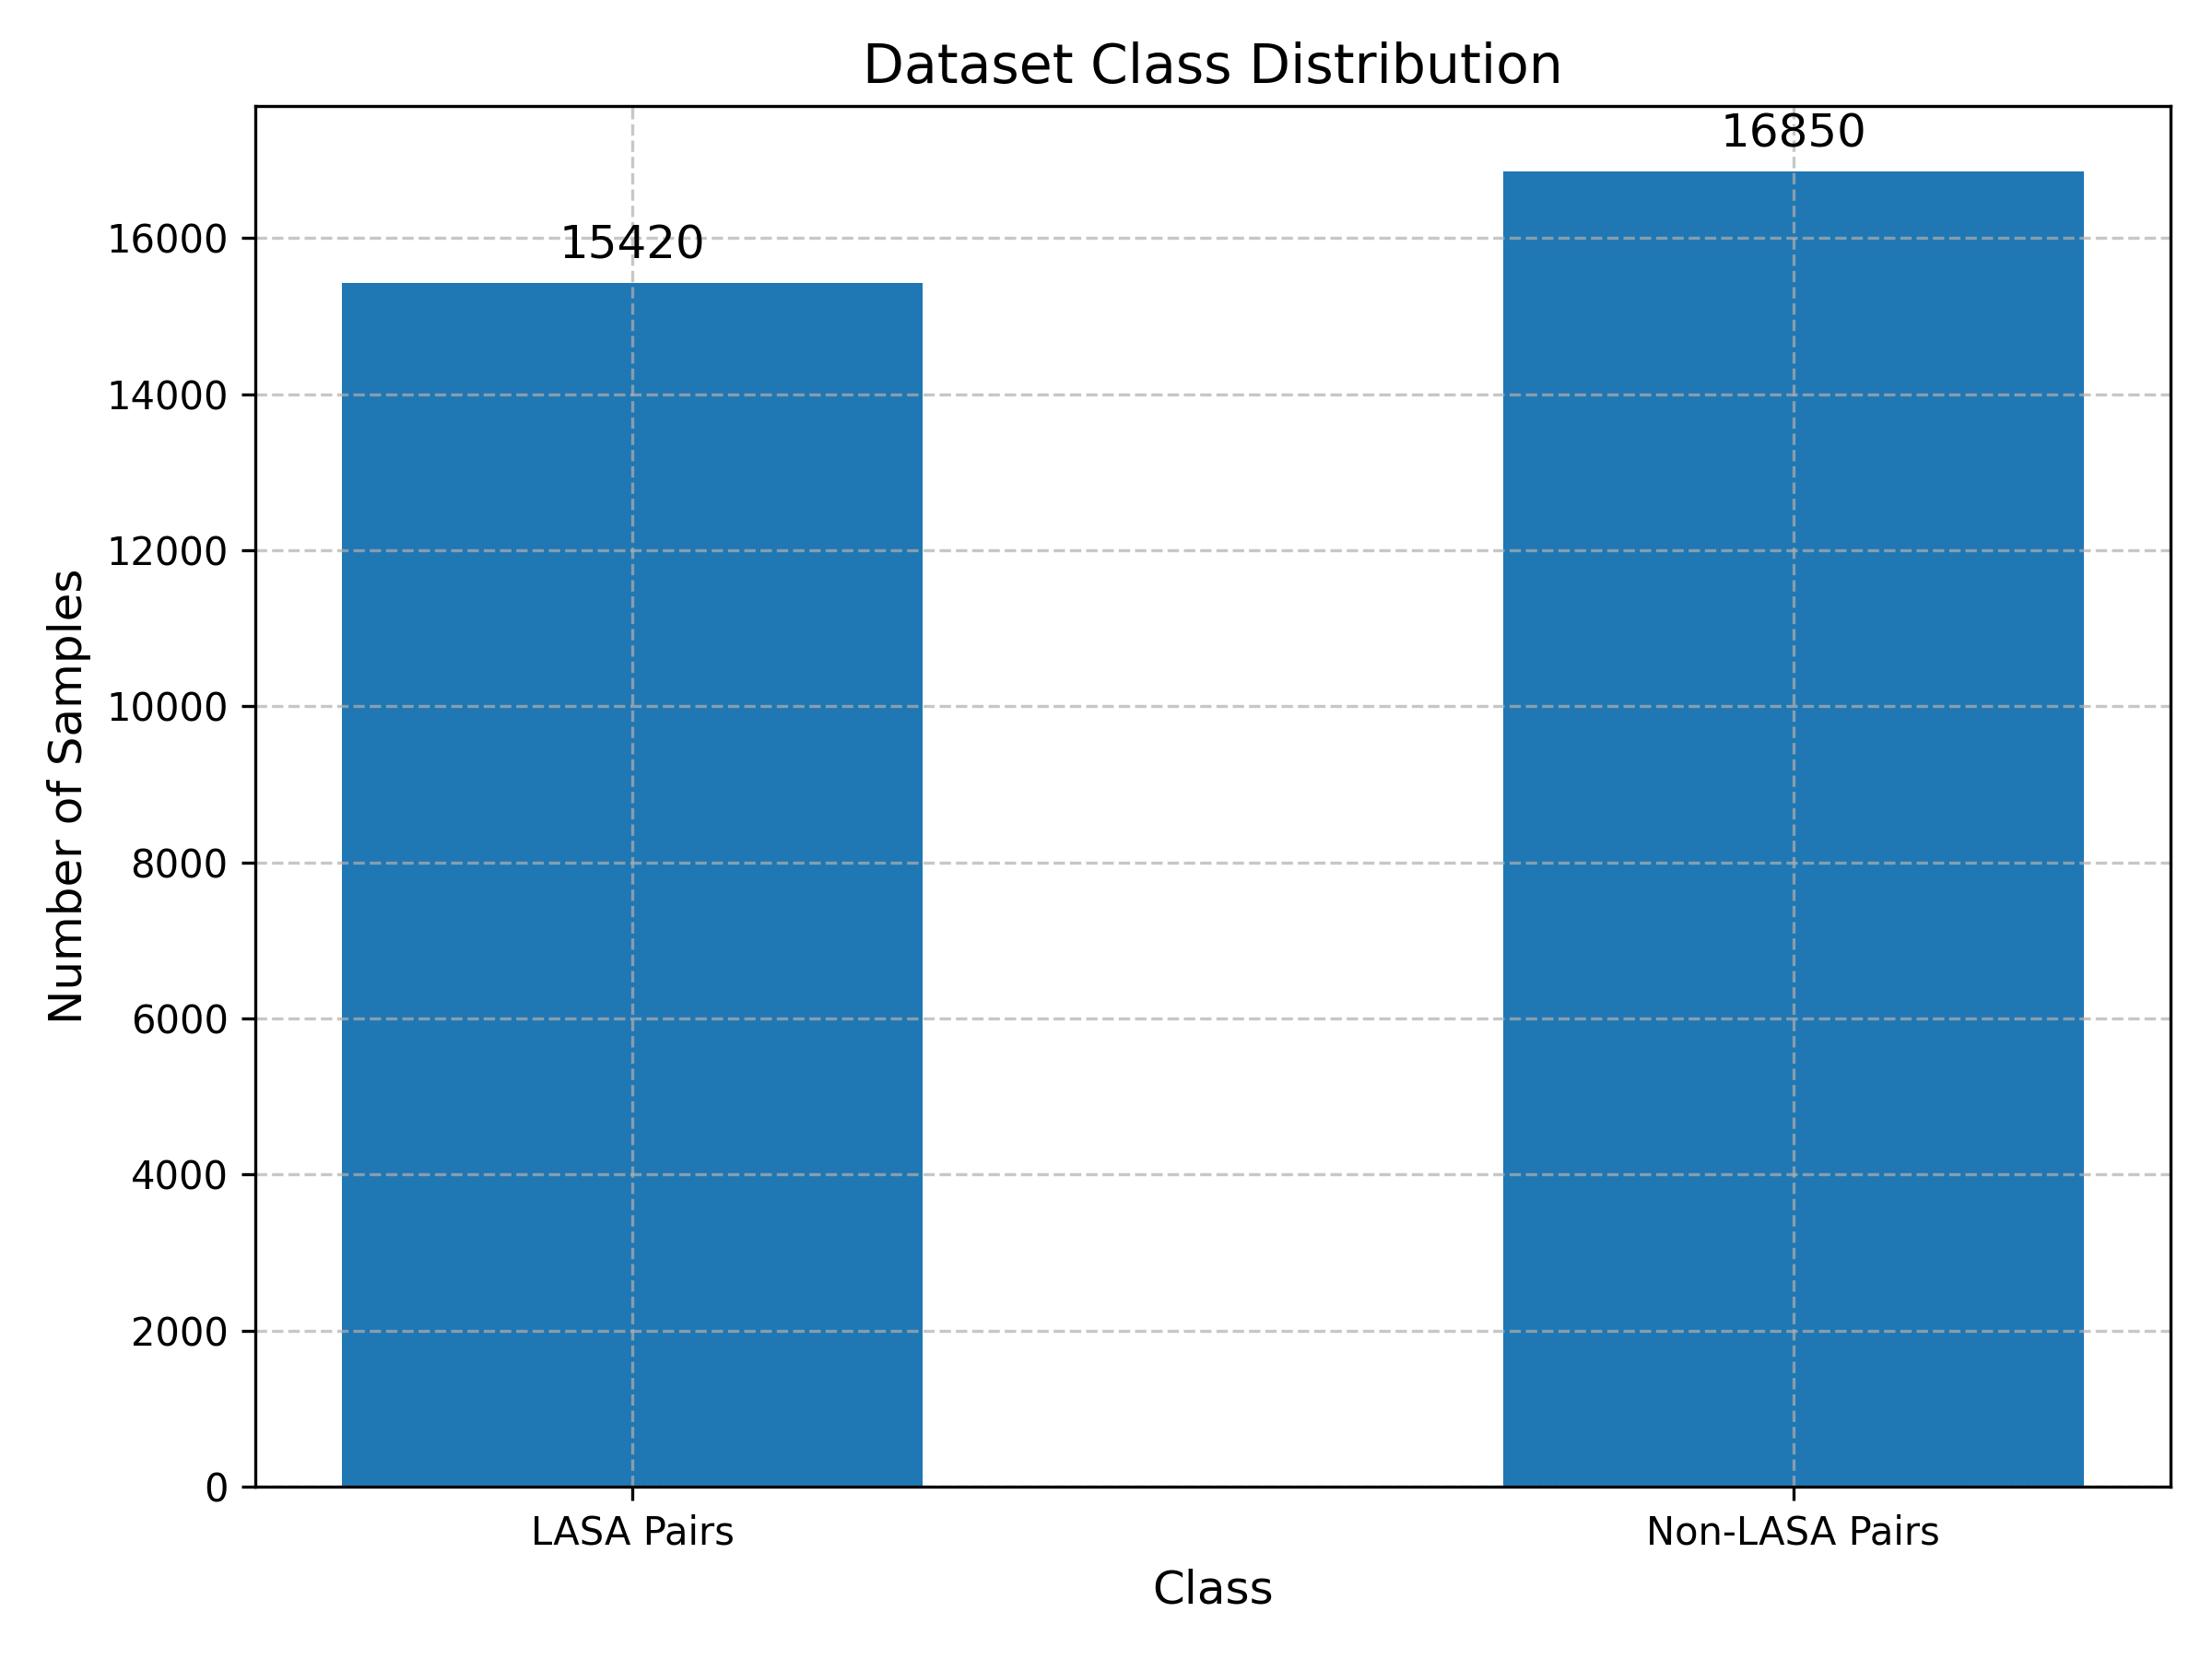
\includegraphics[width=0.8\textwidth]{figures/dataset_distribution.png}
\caption{Class Distribution of the Training Dataset}
\label{fig:dataset-distribution}
\end{figure}

\begin{figure}[h]
\centering
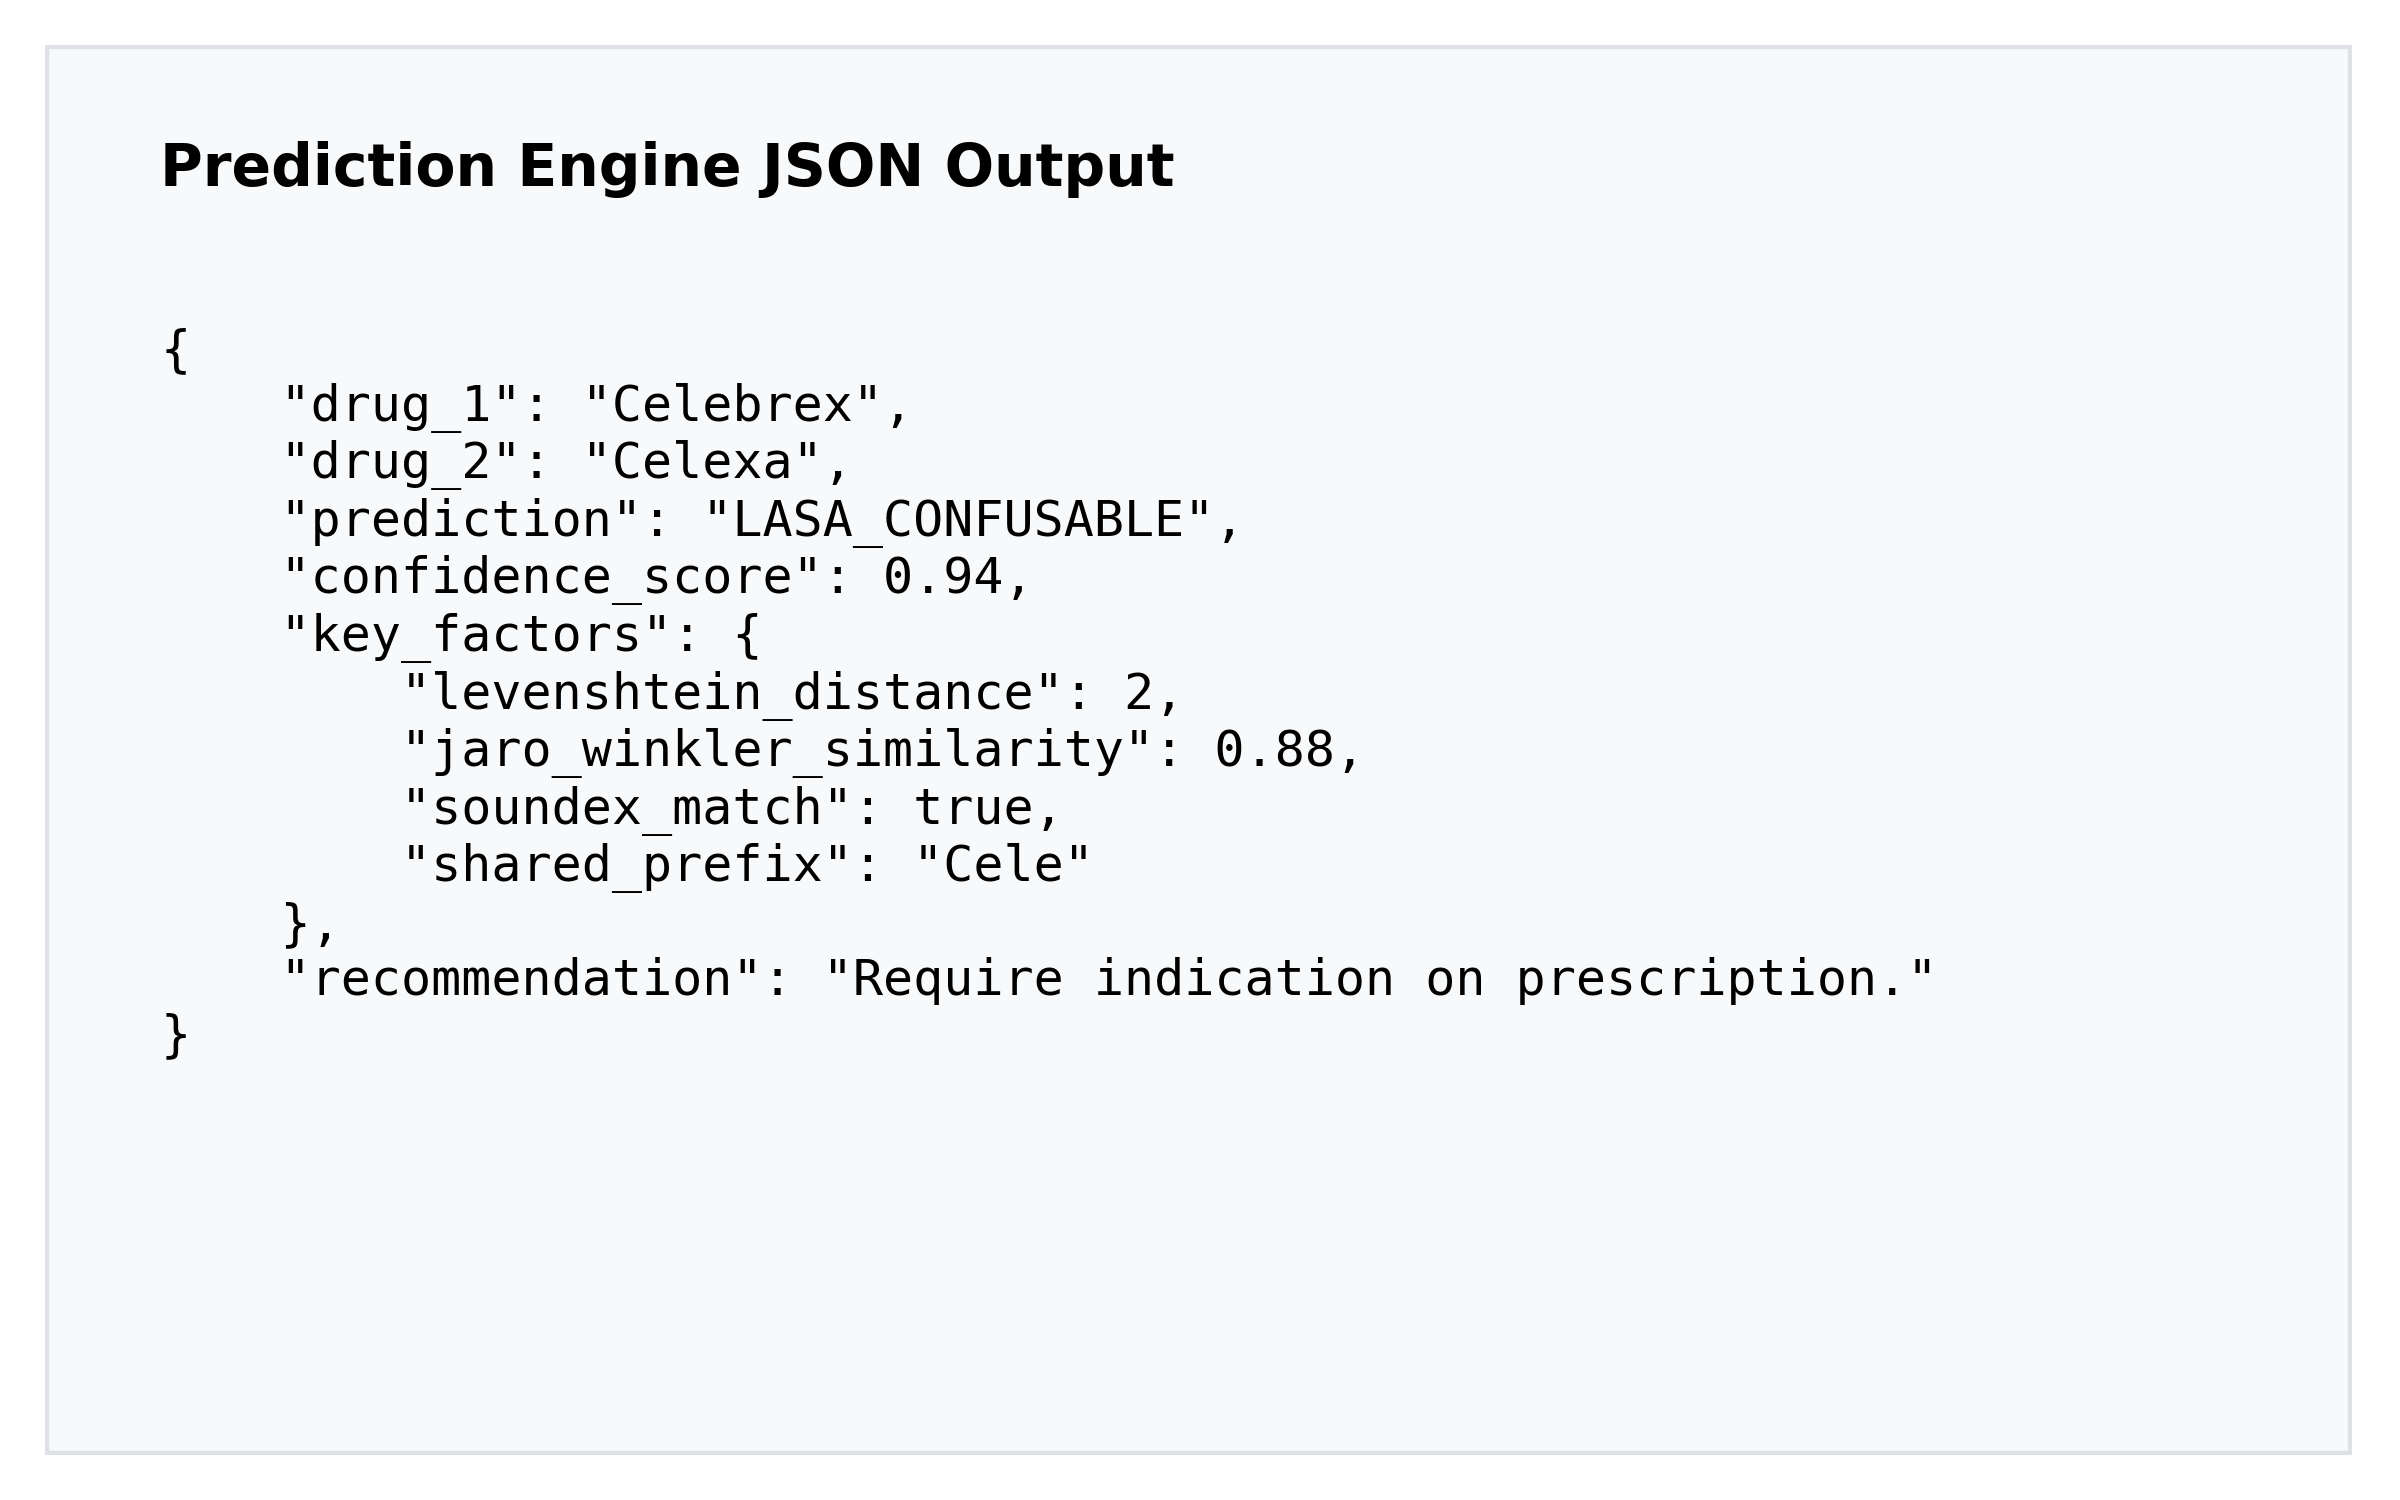
\includegraphics[width=0.8\textwidth]{figures/sample_output.png}
\caption{Sample JSON Output from the Prediction Engine}
\label{fig:sample-output}
\end{figure}

